% CS-327 CEP report, group G2 (meshsync). Skeleton: issue #73. Content: #74, #75.
% Owner: all members. Rules: AGENTS.md; formal requirements: report/README.md.
%
% Builds with Tectonic / XeLaTeX / LuaLaTeX (fontspec) or pdfLaTeX (Overleaf).
%   tectonic main.tex        or        latexmk -pdf main.tex
%
% Formal requirements (course brief §9-§11 and rubric):
%   - at most 10 pages, excluding the rubric title page, references and the code appendix;
%     the build log prints "BODY PAGES: N (limit 10)" and warns when N > 10.
%   - Times New Roman, 12 pt body, 14 pt headings.
%   - the filled-in grading rubric is the title page (no separate title page).
%   - figures and tables labelled and numbered (\caption + \label).
%
% Packages, fonts, layout and macros: preamble.tex (style follows the team's CS-326 SRS).
\documentclass[12pt,a4paper]{article}
% =====================================================================
%  preamble.tex -- packages, page layout and report macros
%  Style follows the team's CS-326 SRS (layout, captions, header, tables, links),
%  adapted to the CS-327 brief: Times New Roman, 12 pt body, 14 pt headings.
%  Common packages only (TeX Live / Tectonic bundle / Overleaf).
% =====================================================================

% ---- Fonts: Times New Roman 12 pt body ---------------------------------
\usepackage{iftex}
\ifPDFTeX
  % pdfLaTeX (Overleaf): newtx is a Times clone.
  \usepackage[T1]{fontenc}
  \usepackage{newtxtext,newtxmath}
  \usepackage{textcomp}
  \input{glyphtounicode}\pdfgentounicode=1   % searchable/copyable text
\else
  % XeTeX (Tectonic) / LuaTeX. Fonts are loaded by FILE NAME only: a lookup by font name
  % (e.g. \IfFontExistsTF{Times New Roman}) makes Tectonic scan every system font through
  % fontconfig, and one malformed system font crashes it (Tectonic panic in fc.rs).
  \usepackage{fontspec}
  % Real Times New Roman: install the font files (Arch: ttf-ms-fonts, which puts
  % times.ttf, timesbd.ttf, timesi.ttf, timesbi.ttf in /usr/share/fonts/TTF/), then set
  % \realtimestrue below. Default: TeX Gyre Termes, a Times clone in the Tectonic bundle.
  \newif\ifrealtimes
  \realtimesfalse
  \newcommand{\timesfontpath}{/usr/share/fonts/TTF/}
  \ifrealtimes
    \setmainfont{times}[
      Path = \timesfontpath,
      Extension = .ttf,
      UprightFont = *,
      BoldFont = *bd,
      ItalicFont = *i,
      BoldItalicFont = *bi]
  \else
    \setmainfont{texgyretermes}[
      Extension = .otf,
      UprightFont = *-regular,
      BoldFont = *-bold,
      ItalicFont = *-italic,
      BoldItalicFont = *-bolditalic]
  \fi
\fi

% ---- Page layout: A4, 1 inch margins (as the SRS) ------------------------
% Paper size and margins are not set by the brief text we have: confirm before submission.
\usepackage[a4paper,margin=1in,headheight=15pt]{geometry}
\setlength{\parindent}{0pt}
\setlength{\parskip}{0.35\baselineskip}
\setlength{\emergencystretch}{2.5em}   % lets TeX loosen a line instead of overrunning the margin

% ---- Tables, figures, colour ------------------------------------------
\usepackage{array,booktabs,longtable,tabularx}
\usepackage{graphicx}
\usepackage{pdfpages}
\usepackage{xcolor}
\usepackage{refcount}
% Captions: bold label as in the SRS, but body size (the brief fixes 12 pt).
\usepackage[labelfont=bf,skip=6pt]{caption}
\definecolor{replink}{RGB}{20,55,120}
\definecolor{repgrey}{gray}{0.40}
\graphicspath{{figures/}{../docs/diagrams/}{../analysis/out/}}

% ---- Float placement: fewer half-empty float pages ---------------------------
\renewcommand{\topfraction}{0.9}\renewcommand{\bottomfraction}{0.6}
\renewcommand{\textfraction}{0.08}\renewcommand{\floatpagefraction}{0.8}
\setcounter{topnumber}{3}\setcounter{totalnumber}{4}

% ---- Headings: 14 pt (brief), compact datasheet style (SRS) ------------------
\usepackage{titlesec}
\setcounter{secnumdepth}{3}
\titleformat{\section}{\fontsize{14}{17}\selectfont\bfseries}{\thesection}{0.7em}{}
% Lower levels stay at body size (12 pt), below the 14 pt heading size.
\titleformat{\subsection}{\normalsize\bfseries}{\thesubsection}{0.7em}{}
\titleformat{\subsubsection}{\normalsize\bfseries\itshape}{\thesubsubsection}{0.7em}{}
\titlespacing*{\section}{0pt}{2.2ex plus 1ex minus .2ex}{0.8ex}
\titlespacing*{\subsection}{0pt}{1.8ex plus 1ex minus .2ex}{0.6ex}
\titlespacing*{\subsubsection}{0pt}{1.5ex plus .8ex minus .2ex}{0.4ex}

% ---- Running header/footer ---------------------------------------------
\usepackage{fancyhdr}
\pagestyle{fancy}
\fancyhf{}
\fancyhead[L]{\small\color{repgrey}meshsync -- CS-327 CEP report}
\fancyhead[R]{\small\color{repgrey}Group G2}
\fancyfoot[C]{\small\thepage}
\renewcommand{\headrulewidth}{0.4pt}
\fancypagestyle{plain}{\fancyhf{}\fancyfoot[C]{\small\thepage}\renewcommand{\headrulewidth}{0pt}}

% ---- Hyperlinks (load late) --------------------------------------------
\PassOptionsToPackage{hyphens}{url}
\usepackage{url}
\Urlmuskip=0mu plus 1mu
\usepackage[colorlinks=true,linkcolor=replink,urlcolor=replink,citecolor=replink,
            bookmarksnumbered=true,pdfstartview=FitH]{hyperref}
\urlstyle{same}
\hypersetup{
  pdftitle={meshsync: a serverless peer-to-peer file synchroniser},
  pdfauthor={M. A. Qazi, M. J. Rao, H. Hanif (CS-327 Group G2)},
  pdfsubject={CS-327 CEP report}}

% =====================================================================
%  Report macros
% =====================================================================

% ---- Inline helpers ------------------------------------------------------
\newcommand{\code}[1]{\texttt{#1}}          % code, paths, message types
\newcommand{\secref}[1]{\ref{sec:#1}}       % section number, hyperlinked

% Visible marker for anything not filled in yet. Search the PDF for "TODO" before submitting.
\newcommand{\TODO}[1]{\textcolor{red}{\textbf{TODO:} #1}}

% ---- Tables ----------------------------------------------------------------
% reptable: longtable wrapper (breaks across pages, header repeats).
%   \begin{reptable}{<column spec>} \caption{..}\label{..}\\ \toprule ... \end{reptable}
% Optional first argument sets the font size; the default keeps body size (12 pt).
\newcommand{\colhead}[1]{\textbf{#1}}
\newcommand{\tablecontinued}{\footnotesize\itshape (continued)}
\newenvironment{reptable}[2][\normalsize]{%
  \par#1\renewcommand{\arraystretch}{1.15}%
  \setlength{\LTpre}{4pt}\setlength{\LTpost}{6pt}%
  \begin{longtable}{@{}#2@{}}}{%
  \end{longtable}\par}

% ---- Figures ----------------------------------------------------------------
% \fitgraphic[maxheight]{file}: natural size, shrunk to \linewidth and to
% maxheight if needed -- never enlarged.
\newsavebox{\repfigbox}
\newcommand{\fitgraphic}[2][0.8\textheight]{%
  \sbox{\repfigbox}{\includegraphics{#2}}%
  \ifdim\wd\repfigbox>\linewidth \sbox{\repfigbox}{\includegraphics[width=\linewidth]{#2}}\fi
  \ifdim\ht\repfigbox>#1\relax \sbox{\repfigbox}{\includegraphics[height=#1]{#2}}\fi
  \usebox{\repfigbox}}
% \repfigure{file}{caption}{label}{maxheight}
\newcommand{\repfigure}[4]{%
  \begin{figure}[!htbp]\centering
    \fitgraphic[#4]{#1}
    \caption{#2}\label{#3}
  \end{figure}}
% \placeholderfigure{todo text}{caption}{label}: boxed slot until the real figure exists.
\newcommand{\placeholderfigure}[3]{%
  \begin{figure}[!htbp]\centering
    \fbox{\parbox[c][4cm][c]{0.9\linewidth}{\centering\TODO{#1}}}
    \caption{#2}\label{#3}
  \end{figure}}

% ---- Notes and references --------------------------------------------------
\newenvironment{repnote}{\par\itshape\leftskip=1.5em\rightskip=1.5em}{\par}
% \refentry{n}{text}: numbered IEEE reference with link target bib:n (no BibTeX run).
\newcommand{\refentry}[2]{%
  \par\noindent{\raggedright\hangindent=2.4em\hangafter=1
  \makebox[2.4em][l]{\hypertarget{bib:#1}{[#1]}}#2\par}\vspace{-0.4\parskip}}
\newcommand{\refcite}[1]{[\hyperlink{bib:#1}{#1}]}


\begin{document}

% ---- Title page: the course's grading rubric (no separate title page) -----------------
% Put the filled-in rubric at report/rubric.pdf (gitignored: we attach it ourselves).
\pagenumbering{gobble}
\IfFileExists{rubric.pdf}{%
  \includepdf[pages=-]{rubric.pdf}%
}{%
  % Shown only when report/rubric.pdf is missing. Replace by placing the filled-in rubric PDF
% at report/rubric.pdf; main.tex then includes it as the title page.
\begin{center}
  \fbox{\parbox{0.9\linewidth}{\centering\vspace{1em}
    {\fontsize{14}{17}\selectfont\bfseries RUBRIC TITLE PAGE GOES HERE}\\[1em]
    \TODO{put the filled-in grading rubric PDF at \texttt{report/rubric.pdf}}\\[1em]
    \begin{tabular}{ll}
      Course  & CS-327 CEP \\
      Group   & G2 \\
      Option  & E (custom, approved deviation) \\
    \end{tabular}\\[1em]
    \begin{tabular}{ll}
      \toprule
      Name & Roll No. \\
      \midrule
      Muhammad Ahmed Qazi & CS-24045 \\
      Mujtaba Jawaid Rao  & CS-24047 \\
      Huzaifa Hanif       & CS-24039 \\
      \bottomrule
    \end{tabular}\vspace{1em}}}
\end{center}
%
}

% ---- Body: counted against the 10-page limit ------------------------------------------
\clearpage
\pagenumbering{arabic}

% !TEX root = ../main.tex
% Section 1. Page budget: about 0.5 page (trimming pass, 2026-11-24).
% Sources: PROJECT_CONTEXT.md §1 (summary), §2 (deviations), §5 (improvements); course brief §5
% (Option E wording). D-numbers: D6 (pure P2P), D10 (CDC), D11 (tagged discovery).
\vspace{0.6pt}
\section{Introduction and the option selected}
\label{sec:intro}

meshsync keeps one shared folder identical on three Linux hosts, with no central server: every
host is an equal peer, and a change on one reaches the others within seconds. We chose a custom
option extending Option~E (file distribution): a peer-to-peer synchroniser with our own protocol on
sockets, UDP broadcast for discovery and TCP for everything else. Instead of a scaling study,
Section~\ref{sec:ftp} compares it with FTP, a client-server protocol, on the same hosts. Each
feature fixes a gap in an existing protocol: only changed chunks travel, unlike FTP, even after an
insert (content-defined chunking); request IDs allow out-of-order replies, unlike HTTP/1.1; many peers
stay in sync continuously, unlike rsync; and an HMAC handshake never sends the secret, unlike FTP's
clear-text password.

\paragraph{Approved deviations.} From our approved proposal, quoted verbatim:

\begin{quote}
Approved deviations (stated in proposal): custom option (extends Option E); R5 capture in plain
mode; no client-server vs P2P scaling comparison.
\end{quote}

% Section 2. Suggested page budget: 1.5 pages (suggestion only).
% Filled by: #74 (R1). Source: docs/PROTOCOL.md (condensed), PROJECT_CONTEXT.md §6.
\section{Protocol specification (R1)}
\label{sec:protocol}

\TODO{filled by \#74: message types, header field formats, legal message order, action on
receipt, status/error codes (from docs/PROTOCOL.md).}

\begin{table}[htbp]
  \centering
  \caption{Protocol message formats.}
  \label{tab:msg-formats}
  \begin{tabular}{lll}
    \toprule
    Message type & Fields & Transport \\
    \midrule
    \multicolumn{3}{c}{\TODO{filled by \#74}} \\
    \bottomrule
  \end{tabular}
\end{table}

% !TEX root = ../main.tex
% Section 3. Suggested page budget: 1.5 pages (suggestion only).
% Filled by: #74 (R3). Sources: docs/diagrams/ (network diagram), data/deploy/README.md
% (3-host deployment session, #67: addresses and host configuration).
\section{System and deployment architecture (R3)}
\label{sec:architecture}

\TODO{filled by \#74: system architecture and the 3-host deployment.}

\placeholderfigure{filled by \#74: network diagram (docs/diagrams/)}{Network diagram of the three-host deployment.}{fig:network}

\begin{reptable}{>{\raggedright\arraybackslash}p{\dimexpr0.3\linewidth-2\tabcolsep\relax}>{\raggedright\arraybackslash}p{\dimexpr0.3\linewidth-2\tabcolsep\relax}>{\raggedright\arraybackslash}p{\dimexpr0.4\linewidth-2\tabcolsep\relax}}
\caption{IP addressing plan.}\label{tab:ip-plan}\\
\toprule
\colhead{Host} & \colhead{Interface} & \colhead{IP address / prefix} \\
\midrule
\endfirsthead
\multicolumn{3}{@{}l}{\tablecontinued}\\
\toprule
\colhead{Host} & \colhead{Interface} & \colhead{IP address / prefix} \\
\midrule
\endhead
\bottomrule
\endlastfoot
\multicolumn{3}{@{}l}{\TODO{filled by \#74 (data/deploy/README.md)}} \\
\end{reptable}

\begin{reptable}{>{\raggedright\arraybackslash}p{\dimexpr0.25\linewidth-2\tabcolsep\relax}>{\raggedright\arraybackslash}p{\dimexpr0.75\linewidth-2\tabcolsep\relax}}
\caption{Configuration of each host.}\label{tab:host-config}\\
\toprule
\colhead{Host} & \colhead{Configuration} \\
\midrule
\endfirsthead
\multicolumn{2}{@{}l}{\tablecontinued}\\
\toprule
\colhead{Host} & \colhead{Configuration} \\
\midrule
\endhead
\bottomrule
\endlastfoot
\multicolumn{2}{@{}l}{\TODO{filled by \#74 (data/deploy/README.md)}} \\
\end{reptable}

% Section 4. Suggested page budget: 1 page (suggestion only).
% Filled by: #74 (R4, transport justification); R2 implementation notes not assigned yet.
% Sources: PROJECT_CONTEXT.md §2 (R2), §4 (D1-D15), §6.1 (transport), src/meshsync/.
\section{Implementation notes (R2, R4)}
\label{sec:implementation}

\TODO{R2 implementation notes: socket API only, no application-protocol libraries (not
assigned to \#74/\#75 yet).}

\subsection{Transport layer justification (R4)}
\label{sec:transport}

\TODO{filled by \#74: per message type, TCP or UDP, justified against reliable transfer,
throughput, timing and security, and what the opposite choice would lose.}

% !TEX root = ../main.tex
% Section 5. Page budget: about 1 page (trimming pass, 2026-11-24).
% Filled by #75 stage 1 (R5). Sources: data/captures/README.md (#68) and data/captures/cap1.pcapng.gz,
% decoded with tshark 4.2.2 and tools/wireshark/meshsync.lua (#87). Every value below was
% read from the capture with tshark (cap1 frame 317 unless stated). MACs in the capture are
% anonymised (scripts/measure/anon_mac.py).
\section{Packet capture and encapsulation analysis (R5)}
\label{sec:capture}

\textbf{Method.} We captured a plain-mode sync of a 100\,MiB file from kratos to defalt with
\code{tshark} on kratos, keeping the first 256 bytes of each frame. Plain mode is our approved R5
deviation, since TLS would hide our messages. MAC addresses were anonymised before commit. Our
Wireshark dissector decodes the meshsync header as its own layer. Figure~\ref{fig:capture} shows one CHUNK\_REQ from defalt.
% tshark -s 256 -f "udp port 47000 or tcp port 47001" on wlp2s0; data/captures/README.md ("How
% they were taken", "Privacy"); tools/wireshark/README.md (D5).
% Figure: Wireshark screenshots by Ahmed (2026-11-25), selected detail lines stacked and
% annotated per layer (layout only; no values changed).

\IfFileExists{figures/capture-chunkreq.png}{%
  \repfigure{capture-chunkreq.png}{One CHUNK\_REQ in Wireshark with our dissector (capture
  \code{cap1}, frame 317), annotated by layer. Selected lines of each header are shown; the red box
  marks our 12-byte header in the packet bytes.}{fig:capture}{0.42\textheight}%
}{%
  \placeholderfigure{Wireshark screenshot of cap1 frame 317, saved as
  report/figures/capture-chunkreq.png}{One CHUNK\_REQ in Wireshark with the meshsync dissector
  (capture \code{cap1}, frame 317), every layer expanded.}{fig:capture}%
}

Each layer adds what the one above lacks: the link header delivers the frame across the Wi-Fi
LAN, IP addresses the other host, TCP reaches our process by port with a reliable, ordered stream,
and our header marks each message's boundary, type and request ID.
% cap1 frame 317: eth.dst/src/type, ip.src/dst/len/ttl/proto/flags.df, tcp.srcport/dstport/seq/
% ack/flags/window_size_value (scale 128)/options, meshsync.* (tshark -V with meshsync.lua).

\textbf{Encapsulation.} Each layer wraps the one above in its own header (Figure~\ref{fig:encap}).
On kratos each header is read by the matching layer and removed: the frame by the network card,
IP and TCP by the kernel, and our header by meshsync. Only the link header changes from hop to hop.

\begin{figure}[H]\centering
  % Encapsulation of one CHUNK_REQ (R5): cap1 frame 317. TikZ fragment, \input by
% report/sections/05-capture.tex. Sizes from tshark: frame.len 154, eth 14, ip.hdr_len 20,
% tcp.hdr_len 32, meshsync header 12, body_len 76 (88 TCP payload, 120 segment, 140 packet).
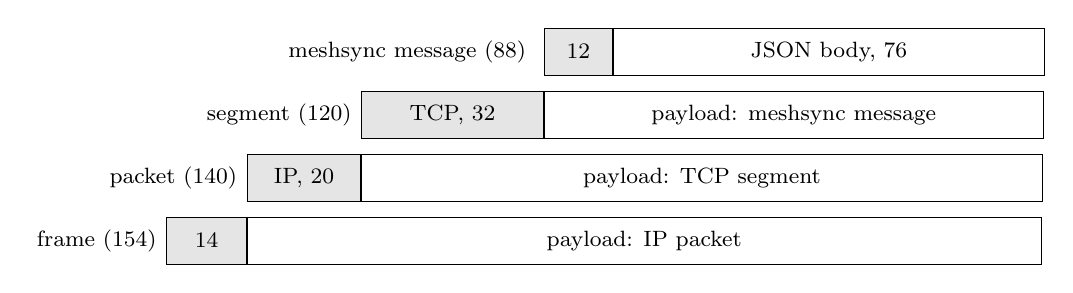
\begin{tikzpicture}[font=\footnotesize, box/.style={draw, minimum height=6mm, inner sep=2pt},
    hd/.style={box, fill=black!10}, pl/.style={box, fill=white}]
  \def\u{0.072} % cm per byte
  % row 4: application message
  \node[hd, minimum width=12*\u cm, anchor=west] (mh) at (6.6,0) {12};
  \node[pl, minimum width=76*\u cm, anchor=west] (mb) at (mh.east) {JSON body, 76};
  \node[anchor=east] at (6.5,0) {meshsync message (88)};
  % row 3: TCP segment
  \node[hd, minimum width=32*\u cm, anchor=east] (th) at (6.6,-0.8) {TCP, 32};
  \node[pl, minimum width=88*\u cm, anchor=west] (tp) at (th.east) {payload: meshsync message};
  \node[anchor=east] at (th.west) {segment (120)};
  % row 2: IP packet
  \node[hd, minimum width=20*\u cm, anchor=east] (ih) at (th.west |- 0,-1.6) {IP, 20};
  \node[pl, minimum width=120*\u cm, anchor=west] (ip) at (ih.east) {payload: TCP segment};
  \node[anchor=east] at (ih.west) {packet (140)};
  % row 1: frame
  \node[hd, minimum width=14*\u cm, anchor=east] (fh) at (ih.west |- 0,-2.4) {14};
  \node[pl, minimum width=140*\u cm, anchor=west] (fp) at (fh.east) {payload: IP packet};
  \node[anchor=east] at (fh.west) {frame (154)};
\end{tikzpicture}

  \caption{Encapsulation of the CHUNK\_REQ in frame 317, in bytes. Grey: each layer's header.}
  \label{fig:encap}
\end{figure}
% Sizes: frame.len 154, ip.len 140, tcp.hdr_len 32, tcp.len 88, meshsync.body_len 76.

\textbf{Overhead.} In this small frame 78 of 154 bytes are headers, only 12 of them ours. Over the
whole 100\,MiB transfer our messages added 0.21\,\% and all headers 5.98\,\%.
% cap1 frame 225: frame.len 1514, tcp.len 1448, CHUNK_DATA body_len 65558. Whole transfer:
% data/captures/README.md ("Header and body overhead").

% !TEX root = ../main.tex
% Section 6. Page budget: part of the 4.25 pages for §5-§10 (report/README.md).
% Filled by #75. Stage 1 (this version): the network baseline only, from data/baseline/ (#70,
% #83). Stage 2 adds the §11 experiments from #77 (analysis/out/, #71).
\section{Performance measurement, results and graphs (R6)}
\label{sec:performance}

\subsection{Network baseline}
\label{sec:baseline}

Before measuring meshsync we measured the network itself on the demo LAN (14 November 2026), in
each direction between the three hosts: round-trip time with \code{ping} (5 runs of 10 echoes;
each run's average is one sample), meshsync's own PING/PONG round trips from a 3-minute
plain-mode run (Table~\ref{tab:rtt}), and the TCP throughput ceiling with \code{iperf3} (5 runs of
10\,s, receiver side, 1\,Mbit = $10^6$ bit; Table~\ref{tab:iperf}). Values are mean $\pm$ sample
standard deviation; ``src $\rightarrow$ dst'' is the side that sends the echo request or the data.
% data/baseline/README.md ("Files", method settings, "Results"); summary.csv; pingpong.csv.

\begin{reptable}{>{\raggedright\arraybackslash}p{\dimexpr0.30\linewidth-2\tabcolsep\relax}>{\raggedright\arraybackslash}p{\dimexpr0.35\linewidth-2\tabcolsep\relax}>{\raggedright\arraybackslash}p{\dimexpr0.35\linewidth-2\tabcolsep\relax}}
\caption{Round-trip time between the hosts (ms).}\label{tab:rtt}\\
\toprule
\colhead{src $\rightarrow$ dst} & \colhead{\code{ping} (n = 5 runs)} & \colhead{meshsync PING/PONG (n)} \\
\midrule
\endfirsthead
\multicolumn{3}{@{}l}{\tablecontinued}\\
\toprule
\colhead{src $\rightarrow$ dst} & \colhead{\code{ping} (n = 5 runs)} & \colhead{meshsync PING/PONG (n)} \\
\midrule
\endhead
\bottomrule
\endlastfoot
kratos $\rightarrow$ defalt & 9.70 $\pm$ 10.27 & 10.91 $\pm$ 5.59 (20) \\
defalt $\rightarrow$ kratos & 8.55 $\pm$ 3.42 & 10.87 $\pm$ 4.81 (20) \\
kratos $\rightarrow$ minipc & 68.02 $\pm$ 25.97 & 71.82 $\pm$ 29.38 (21) \\
minipc $\rightarrow$ kratos & 14.24 $\pm$ 10.78 & 13.19 $\pm$ 3.56 (21) \\
minipc $\rightarrow$ defalt & 17.34 $\pm$ 13.81 & 17.15 $\pm$ 14.62 (21) \\
defalt $\rightarrow$ minipc & 56.53 $\pm$ 5.61 & 35.98 $\pm$ 20.42 (20) \\
\end{reptable}
% ping: data/baseline/summary.csv (metric rtt_ms, n 5). PING/PONG: data/baseline/pingpong.csv,
% mean and sample sd per (host, peer) computed from its rtt_ms rows (n 20-21).

\begin{reptable}{>{\raggedright\arraybackslash}p{\dimexpr0.4\linewidth-2\tabcolsep\relax}>{\raggedright\arraybackslash}p{\dimexpr0.6\linewidth-2\tabcolsep\relax}}
\caption{TCP throughput ceiling, \code{iperf3} (n = 5 runs).}\label{tab:iperf}\\
\toprule
\colhead{src $\rightarrow$ dst} & \colhead{Throughput (Mbit/s)} \\
\midrule
\endfirsthead
\multicolumn{2}{@{}l}{\tablecontinued}\\
\toprule
\colhead{src $\rightarrow$ dst} & \colhead{Throughput (Mbit/s)} \\
\midrule
\endhead
\bottomrule
\endlastfoot
kratos $\rightarrow$ defalt & 16.58 $\pm$ 0.78 \\
defalt $\rightarrow$ kratos & 7.66 $\pm$ 1.26 \\
kratos $\rightarrow$ minipc & 14.29 $\pm$ 3.62 \\
minipc $\rightarrow$ kratos & 27.59 $\pm$ 1.41 \\
minipc $\rightarrow$ defalt & 10.45 $\pm$ 2.63 \\
defalt $\rightarrow$ minipc & 10.38 $\pm$ 1.34 \\
\end{reptable}
% data/baseline/summary.csv (metric throughput_mbps, n 5).

\textbf{Interpreting the RTT.} Each round trip is the sum of the nodal delays
$d_\mathrm{proc} + d_\mathrm{queue} + d_\mathrm{trans} + d_\mathrm{prop}$ on every hop, and here every
packet crosses the air twice (sender to access point to receiver) on one shared channel. On one
LAN $d_\mathrm{prop}$ is negligible, and $d_\mathrm{trans}$ is small for short echo frames, so the
spread comes from queueing and waiting for the channel. The data show this: the fastest single
echo in any run took 2.1\,ms, run averages reach 98.6\,ms, single echoes up to 348.8\,ms, and the
standard deviations are often comparable to the means. Three runs lost one of their ten echoes. The
clearest pattern is that traffic \emph{to} minipc is slow (57--68\,ms) while traffic \emph{from}
it is fast (14--17\,ms): Wi-Fi power saving is on for minipc, so the access point holds frames
for it until its radio wakes. That waiting is queueing delay, not distance. meshsync's PING/PONG
agrees with \code{ping} within 4\,ms in five of six directions, usually slightly above it,
which fits our own extra $d_\mathrm{proc}$ (Python, framing, the reader thread). The exception, defalt $\rightarrow$
minipc (36 vs 57\,ms), also waits on minipc's sleep cycle, and the high standard deviation (20\,ms)
reflects when each probe happened to arrive. The \code{iperf3} ceiling is 7.7--27.6\,Mbit/s and
depends on direction (defalt sends at 7.7 but receives at 16.6\,Mbit/s): this is the upper bound
for any meshsync transfer between these hosts.
% data/baseline/rtt.csv: min(min_ms) 2.077 (defalt->kratos run 2), max(avg_ms) 98.608
% (kratos->minipc run 5), max(max_ms) 348.817 (minipc->defalt run 4), loss_pct 10 in 3 runs.
% Power save and the defalt->minipc explanation: data/baseline/README.md ("Anomalies").
% PROJECT_CONTEXT.md §11 (delay model).

\subsection{Experiments}
\label{sec:experiments}

\textbf{Method.} We ran the §11 conditions on the same three hosts (18--19 November 2026), with
kratos as the driver and source and minipc and defalt as receivers, each condition 5 times. The
workload is set A: a 100\,MiB file (104\,857\,600 bytes), then a 1\,KiB overwrite (delta) or a 1\,KiB
insert at offset 0 (fixed vs content-defined chunking). Impairment is \code{tc netem} on kratos's
Wi-Fi interface: 5\,\% loss, or 50\,ms added delay. For each run, the receivers' values are averaged
first; we then report mean $\pm$ sample standard deviation over the n = 5 runs, as
\code{analysis/analyze.py} computes it. Throughput is chunk bytes divided by transfer time, in MB/s
($10^6$ bytes). One TLS row that \code{analyze.py} flags as a duplicate fetch (\#60) is excluded.
Table~\ref{tab:experiments} gives the results; Figures~\ref{fig:exp-full-delta}
and~\ref{fig:exp-impaired} show two of them. The chunk-size condition (16/64/256\,KiB) was not
run.
% data/README.md (§11 multi-host results: setup, interruptions, tls/run4 flagged);
% scripts/measure/run.py impaired_profiles, LOSS_PCT_DEFAULT 5, DELAY_MS_DEFAULT 50 (hosts.py
% --loss-pct/--delay-ms defaults; data/README.md records no other value); analysis/README.md
% (statistics, throughput). Tables: analysis/out/<experiment>.md from analysis/analyze.py.

\begin{reptable}{>{\raggedright\arraybackslash}p{\dimexpr0.22\linewidth-2\tabcolsep\relax}>{\raggedright\arraybackslash}p{\dimexpr0.12\linewidth-2\tabcolsep\relax}>{\raggedright\arraybackslash}p{\dimexpr0.22\linewidth-2\tabcolsep\relax}>{\raggedright\arraybackslash}p{\dimexpr0.24\linewidth-2\tabcolsep\relax}>{\raggedright\arraybackslash}p{\dimexpr0.20\linewidth-2\tabcolsep\relax}}
\caption{§11 conditions, mean $\pm$ sd over n = 5 runs.}\label{tab:experiments}\\
\toprule
\colhead{Condition} & \colhead{Variant} & \colhead{Transfer time (s)} & \colhead{Chunk bytes received} & \colhead{Throughput (MB/s)} \\
\midrule
\endfirsthead
\multicolumn{5}{@{}l}{\tablecontinued}\\
\toprule
\colhead{Condition} & \colhead{Variant} & \colhead{Transfer time (s)} & \colhead{Chunk bytes received} & \colhead{Throughput (MB/s)} \\
\midrule
\endhead
\bottomrule
\endlastfoot
1 Full vs delta & full & 227.5 $\pm$ 74.99 & 104\,874\,436 & 0.5116 $\pm$ 0.1564 \\
 & delta & 5.204 $\pm$ 10.92 & 75\,667 & 0.3633 $\pm$ 0.3376 \\
2 Fixed vs CDC (insert) & fixed & 143.1 $\pm$ 49.58 & 104\,877\,836 & 0.8572 $\pm$ 0.4003 \\
 & CDC & 0.3006 $\pm$ 0.4061 & 66\,594 & 0.5789 $\pm$ 0.3944 \\
3 Sources & 1 source & 73.33 $\pm$ 30.9 & 104\,894\,652 $\pm$ 45\,205 & 1.66 $\pm$ 0.7107 \\
 & 2 sources & 66.05 $\pm$ 10.22 & 104\,874\,436 & 1.617 $\pm$ 0.2347 \\
5 Link & clean & 116.4 $\pm$ 33.57 & 104\,874\,436 & 1.031 $\pm$ 0.2897 \\
 & 5\,\% loss & 474.2 $\pm$ 143.7 & 104\,874\,436 & 0.2352 $\pm$ 0.05852 \\
 & +50\,ms delay & 118.8 $\pm$ 27.07 & 104\,874\,436 & 0.946 $\pm$ 0.2376 \\
6 Security & plain & 102.9 $\pm$ 16.81 & 104\,874\,436 & 1.055 $\pm$ 0.1655 \\
 & TLS & 90.76 $\pm$ 19.55 & 105\,160\,119 $\pm$ 620\,599 & 1.23 $\pm$ 0.2855 \\
\end{reptable}
% analysis/out/{full_delta,fixed_cdc,sources,impaired,tls}.md (chunk bytes sd 0 except where
% shown; 1 source: 104,894,652 +- 45,205). Connection setup time (tls.md): plain 0.6517 +- 1.078 s,
% TLS 0.2537 +- 0.05434 s.

\begin{figure}[!htbp]\centering
  \begin{minipage}[t]{0.48\linewidth}\centering
    \fitgraphic[0.27\textheight]{exp-full-delta.pdf}
    \caption{Chunk bytes received, full copy vs delta (log scale, n = 5, $\pm$1 sd).}
    \label{fig:exp-full-delta}
  \end{minipage}\hfill
  \begin{minipage}[t]{0.48\linewidth}\centering
    \fitgraphic[0.27\textheight]{exp-impaired.pdf}
    \caption{Transfer time of the 100\,MiB file: clean, 5\,\% loss, +50\,ms delay (n = 5, $\pm$1 sd).}
    \label{fig:exp-impaired}
  \end{minipage}
\end{figure}
% report/figures/exp-full-delta.pdf, exp-impaired.pdf: copies of analysis/out/full_delta.pdf,
% impaired.pdf (analysis/analyze.py).

\textbf{RTT, throughput and the representative operation.} RTT is in Table~\ref{tab:rtt}
(5 runs of \code{ping}, and 20--21 meshsync PING/PONG samples per direction). The representative
operation, syncing the 100\,MiB file to two receivers, took $116.4 \pm 33.6$\,s on the clean link
(condition 5), about $1.03$\,MB/s or 8.2\,Mbit/s. That is about 50--58\,\% of the \code{iperf3}
ceiling from kratos (14.29\,Mbit/s to minipc, 16.58 to defalt; Table~\ref{tab:iperf}). The ceiling is
per pair, and both receivers share one Wi-Fi channel with the source, so it is not additive.

\textbf{Explaining the results with $d_\mathrm{nodal}$.} For the full 100\,MiB transfers,
$d_\mathrm{trans}$ dominates: 104.9\,MB at about 1\,MB/s takes about 100\,s, while a round trip is tens
of milliseconds. The Wi-Fi channel is the bottleneck, and queueing behind it ($d_\mathrm{queue}$)
explains the large run-to-run spread. For delta sync and CDC after an insert, only 75\,667 and 66\,594
chunk bytes cross the network, so $d_\mathrm{trans}$ almost disappears (every run but one under 1.4\,s) and the
remaining time is a few request/reply round trips plus our own $d_\mathrm{proc}$ (hashing, index
compare). 5\,\% loss makes the transfer 4.1 times slower in this batch (2.1 times in a later batch on a better night, Section~\ref{sec:ftp}): lost segments must be retransmitted and TCP
shrinks its congestion window, which shows up as extra waiting, not as distance; the same loss is
behind the 402 retransmissions in Section~\ref{sec:failure}. Adding 50\,ms of delay, a
$d_\mathrm{prop}$-like term, has no clear effect ($118.8 \pm 27.1$ vs $116.4 \pm 33.6$\,s): at
1.031\,MB/s, 50\,ms holds about 52\,KB in flight, far below what our pipelining keeps outstanding
(8 outstanding CHUNK\_REQs per peer $\times$ 64\,KiB average chunk, about 524\,KB), so the link stays busy. Two
sources instead of one give no clear gain ($66.1 \pm 10.2$ vs $73.3 \pm 30.9$\,s): the sources share
the same air time, so the bottleneck does not move. TLS shows no measurable cost: its throughput
($1.23 \pm 0.29$\,MB/s) and setup time ($0.25 \pm 0.05$\,s) are within the spread of plain mode
($1.06 \pm 0.17$\,MB/s, $0.65 \pm 1.08$\,s), because encryption adds a little $d_\mathrm{proc}$ on a link
whose $d_\mathrm{trans}$ is far larger.
% 104874436 B / 1.031e6 B/s = 102 s; 474.2 / 116.4 = 4.07; 1.031e6 x 0.05 = 51,550 B;
% MAX_OUTSTANDING_PER_PEER 8 x CDC_AVG 64 KiB = 524,288 B (constants.py); 1.031 MB/s x 8 = 8.25
% Mbit/s; 8.25/14.29 = 0.58, 8.25/16.58 = 0.50. Per-run values: data/<experiment>/run*.csv.

\textbf{Anomalies.} (1) The same 100\,MiB operation took $227.5 \pm 75.0$\,s in condition 1,
$143.1 \pm 49.6$\,s in condition 2 and $102.9 \pm 16.8$\,s in condition 6: a factor of two between blocks
of one batch. defalt's Wi-Fi was lossy during the batch (25--83\,\% ping loss from kratos) and its power
saving was turned off part-way, so link quality changed over time; byte counts did not. (2) Delta's
standard deviation exceeds its mean ($5.2 \pm 10.9$\,s) because run 4 took 21.7 and 27.8\,s on the two
receivers while every other run took under 1\,s; the CSVs do not show the cause. (3) Plain mode's
setup time ($0.65 \pm 1.08$\,s) comes from one 5.075\,s value (run 5, minipc); the other nine are
0.045--0.364\,s. (4) TLS received more chunk bytes than the file size: besides the excluded run 4,
defalt in run 5 received 107\,665\,543 bytes, a duplicate fetch (\#60) that \code{analyze.py} does not
flag. (5) TLS was not slower than plain; on this network the difference is inside the spread. (6) The 4.1 times loss slowdown of this batch fell to 2.1 times when rerun on the FTP night (Section~\ref{sec:ftp}): the Wi-Fi, not the protocol.
% data/README.md (lossy defalt, power saving); data/full_delta/run4.csv (delta 21.706522,
% 27.767192 s); data/tls/run5.csv (plain minipc setup_s 5.075; tls defalt chunk_bytes 107665543).

\textbf{Limitations.} All runs used one Wi-Fi network whose quality changed during the batch, so
time differences smaller than the spread mean ``no clear effect''. n = 5 runs gives wide intervals,
and two receivers are averaged per run. Times are measured on each receiver from the first
NOTIFY with a 0.5\,s polling step, so sub-second values are coarse. The chunk-size condition and
Wi-Fi vs wired were not run. Host clocks differ (kratos logs are 5\,h ahead), which is why we never
compare times across hosts. The captures in Section~\ref{sec:capture} keep only 256 bytes per
frame, so they give counts and headers, not payload timings.
% data/README.md; data/<experiment>/run*.csv (e2e_from first_notify, poll_s 0.5);
% data/captures/README.md (snaplen 256, kratos clock).

\subsection{Comparison with FTP}
\label{sec:ftp}

To test our claims against an existing protocol (PROJECT\_CONTEXT.md §5) we measured plain FTP on
the same three hosts, file and edits (21 November 2026): kratos ran vsftpd, and minipc and defalt
downloaded at the same time with Python's \code{ftplib}, checking each file's SHA-256 afterwards.
Each run has four variants: the full 100\,MiB file, the file after the 1\,KiB overwrite, after the
1\,KiB insert at offset 0, and the full file under 5\,\% netem loss on kratos. To compare times
fairly, meshsync's link condition (clean, 5\,\% loss, +50\,ms) was rerun right after the FTP batch
on the same night. Table~\ref{tab:ftp} gives mean $\pm$ sd over n = 5 runs, the two receivers
averaged per run, as computed by \code{analyze.py}.
% data/ftp/README.md (setup, variants, same-night batch, times 22:16-23:32 and 23:59-01:23);
% analysis/analyze.py on data/ftp/run*.csv and data/ftp/meshsync_same_night/run*.csv.

\begin{reptable}{>{\raggedright\arraybackslash}p{\dimexpr0.20\linewidth-2\tabcolsep\relax}>{\raggedright\arraybackslash}p{\dimexpr0.20\linewidth-2\tabcolsep\relax}>{\raggedright\arraybackslash}p{\dimexpr0.16\linewidth-2\tabcolsep\relax}>{\raggedright\arraybackslash}p{\dimexpr0.20\linewidth-2\tabcolsep\relax}>{\raggedright\arraybackslash}p{\dimexpr0.24\linewidth-2\tabcolsep\relax}}
\caption{FTP vs meshsync on the same hosts (mean $\pm$ sd, n = 5).}\label{tab:ftp}\\
\toprule
\colhead{Case} & \colhead{FTP time (s)} & \colhead{FTP bytes} & \colhead{meshsync time (s)} & \colhead{meshsync chunk bytes} \\
\midrule
\endfirsthead
\multicolumn{5}{@{}l}{\tablecontinued}\\
\toprule
\colhead{Case} & \colhead{FTP time (s)} & \colhead{FTP bytes} & \colhead{meshsync time (s)} & \colhead{meshsync chunk bytes} \\
\midrule
\endhead
\bottomrule
\endlastfoot
Full file, clean & 106.5 $\pm$ 32.5 & 104\,857\,600 & 162.8 $\pm$ 14.0$^{a}$ & 104\,874\,436 \\
Full file, 5\,\% loss & 248.9 $\pm$ 56.2 & 104\,857\,600 & 346.3 $\pm$ 59.0$^{a}$ & 104\,881\,052 \\
Loss $\div$ clean & 2.3$\times$ & & 2.1$\times$$^{a}$ & \\
1\,KiB overwrite & 88.5 $\pm$ 17.3 & 104\,857\,600 & 5.2 $\pm$ 10.9$^{b}$ & 75\,667 \\
1\,KiB insert at 0 & 87.8 $\pm$ 33.4 & 104\,858\,624 & 0.30 $\pm$ 0.41$^{b}$ & 66\,594 \\
\end{reptable}
{\footnotesize $^{a}$\,Same night as FTP. $^{b}$\,Main batch (Table~\ref{tab:experiments}): delta sync and CDC; not rerun on the FTP night, so compare bytes, not times.\par}
% FTP: analysis of data/ftp/run*.csv (full 106.5 +- 32.53, loss 248.9 +- 56.16, overwrite
% 88.5 +- 17.28, insert 87.83 +- 33.42; bytes sd 0). meshsync same night:
% data/ftp/meshsync_same_night (clean 162.8 +- 14.03, loss 346.3 +- 59.04, loss chunk bytes
% 104,881,052 +- 14,794). 248.9/106.5 = 2.34; 346.3/162.8 = 2.13.

\textbf{What the comparison shows.} After a small edit FTP downloads the whole file again: 1\,386
times the bytes meshsync sent after the overwrite, and 1\,575 times after the insert, because FTP has
no delta transfer. For a fresh full copy FTP was faster on the same night (106.5 vs 162.8\,s): one
plain TCP stream with no chunking, hashing or per-chunk requests, so less $d_\mathrm{proc}$ and fewer
round trips. meshsync's advantage is after edits, in authentication and in integrity, not in raw bulk
speed. Loss hurt both about equally on the same night (2.1 vs 2.3 times the clean time), so the 4.1
times of the main batch (Table~\ref{tab:experiments}) came from that night's worse Wi-Fi, not from
the protocol. A capture of one FTP download (not committed, because it holds the test password)
shows the weaknesses §5 lists: \code{USER} and \code{PASS} in plain text (frames 6 and 9), and two TCP
connections per transfer, the control connection on port 21 (28 frames) and a separate passive data
connection on port 40029 (77\,918 frames). meshsync sends only nonces and MACs in its handshake
(Section~\ref{sec:failure}), uses one connection per peer pair, and checks SHA-256 per chunk, while
the FTP clients had to compare SHA-256 themselves.
% 104,857,600 / 75,667 = 1,385.8; 104,858,624 / 66,594 = 1,574.6. Capture: data/ftp/README.md
% ("What the capture shows").

% Section 7. Suggested page budget: 0.75 page (suggestion only).
% Filled by: #75 (brief §6). Source: PROJECT_CONTEXT.md §12, numbers from analysis/out/.
\section{Design tensions and engineering justification}
\label{sec:tensions}

\TODO{filled by \#75: at least three design tensions, each with our position and our own
numbers.}

% !TEX root = ../main.tex
% Section 8. Page budget: about 0.5 page (trimming pass, 2026-11-24).
% Sources: analysis/out/savings.md (analyze.py on data/full_delta, data/fixed_cdc); PROJECT_CONTEXT.md
% §13 (10,000 users x 20 edits/day, counter-weight); energy: Aslan et al. 2018, reference [1].
% Arithmetic: 200,000 x 105,183,306 B = 21,036.7 GB/day; 200,000 x 171,836 B = 34.4 GB/day;
% saved 21,002.3 GB/day x 365 = 7,665,837 GB/year; x 0.06 kWh/GB = 1,260 kWh/day, 459,950 kWh/year.
% CDC vs fixed after insert: 99.94 % chunk data, 99.85 % all bytes (162,562 vs 105,122,508).
\section{Sustainability and efficiency analysis}
\label{sec:sustainability}

\begin{itemize}[leftmargin=*,itemsep=1pt,topsep=2pt]
  \item \textbf{Bytes saved:} after a 1\,KiB edit to the 100\,MiB file, 171\,836 bytes instead of
  105\,183\,306, counting all traffic: 99.84\,\% less (99.85\,\% for chunking after an insert).
  \item \textbf{At scale (illustration):} 10\,000 users making 20 such edits a day, each to one peer,
  is 34\,GB a day instead of 21\,037\,GB: about 7.67\,PB a year saved.
  \item \textbf{Energy:} at 0.06\,kWh per GB (Aslan et al., 2015 estimate \refcite{1}), about
  1\,260\,kWh a day, or 460\,MWh a year. Orders of magnitude only: few edits touch 100\,MiB files.
  \item \textbf{Counter-weight:} CPU we did not measure, hashing every scanned file and a rolling
  hash over every byte.
\end{itemize}

% !TEX root = ../main.tex
% Section 9. Page budget: part of the 4.25 pages for §5-§10 (report/README.md).
% Filled by #75 stage 1 (R7). Sources: PROJECT_CONTEXT.md §10, docs/PROTOCOL.md,
% data/captures/README.md and cap2-cap5 (+ logs, #68), tests/integration/ (#62, #63).
% Frame numbers and counts from tshark 4.2.2 with tools/wireshark/meshsync.lua. Log times are
% defalt's (UTC); kratos logs are 5 h ahead (data/captures/README.md), converted where quoted.
\section{Behaviour under failure (R7)}
\label{sec:failure}

For each failure scenario we give the designed behaviour, what happened on the real hosts, and
the evidence (captures are kratos's view, taken between kratos and defalt; Section~\ref{sec:capture}).

\textbf{Wrong secret} (designed: the HMAC checks reject the peer, ERROR 0x04, close). The secret
is checked twice. First, discovery: kratos's ANNOUNCEs carry a tag made with a different secret,
so defalt drops each one at receive rule~3 and never dials. \code{cap2} has 14 datagrams
(12 ANNOUNCE, 2 LEAVE) and no TCP frame at all; defalt logs
\code{drop D5A6E688 from 192.168.100.92: bad tag} every 5\,s. Second, with a static peer
(\code{--peer}) to reach the TCP handshake (\code{cap2b}): HELLO (frame 6) $\rightarrow$
HELLO\_ACK (8) $\rightarrow$ ERROR \code{\{"code": 4, "msg": "AUTH\_FAILED: bad mac\_r"\}} (10)
$\rightarrow$ FIN from both sides (11, 12). The dialler, defalt, detects the wrong \code{mac\_r}
first (log 13:41:33: \code{initiator handshake failed: AUTH\_FAILED: bad mac\_r}). The attempt
runs four times in the capture, about every 5\,s, and no meshsync message beyond the handshake is
ever sent.
% cap2: 14 frames, 0 tcp; disc types from meshsync.disc.type; cap2-defalt.log 13:38:53-.
% cap2b frames 6/8/10/11/12 and 20/22/24 (11.77 s); 4 x HELLO, 4 x HELLO_ACK, 4 x ERROR;
% cap2b-defalt.log 13:41:33,557. PROTOCOL.md §3.4 rule 3, §5.2, §10 (0x04 fatal).

\textbf{Spoofed or replayed ANNOUNCE} (designed: dropped, bad tag or stale \code{ts}). The bad-tag
case is the one above. The replay check also fired on real traffic: during \code{cap1} defalt
dropped two of kratos's ANNOUNCEs (\code{drop 953B75EA from 192.168.100.92: replay ts 1794662842},
13:27:24). kratos's own timestamps strictly increase in the capture, so defalt most likely
received the same broadcast twice over Wi-Fi, and the check dropped the copy as designed. A
spoofed and a replayed datagram are also tested on localhost
(\code{test\_spoofed\_and\_replayed\_announce\_dropped}).
% cap1-defalt.log (2 "replay ts" lines); data/captures/README.md ("Observations");
% tests/integration/test_failures.py.

\textbf{Untrusted certificate} (designed: TLS alert, close). defalt used a certificate from a
different CA. In \code{cap3}: Client Hello from defalt (frame 7) $\rightarrow$ Server Hello (9)
$\rightarrow$ Alert, level Fatal, description Unknown CA, from defalt (14). The handshake fails
before any meshsync message, and repeats every 5\,s (alerts in frames 14, 27, 40 and 53; no meshsync
message in the whole capture). defalt logs \code{TLS handshake failed (client side):
[SSL: CERTIFICATE\_VERIFY\_FAILED]} (13:55:31) and kratos \code{tlsv1 alert unknown ca}. A TLS/plain
mode mismatch is tested on localhost (\code{test\_tls\_plain\_mode\_mismatch\_closed}).
% cap3: tls.alert_message level 2, desc 48 (Unknown CA) from 192.168.100.80 in frames
% 14/27/40/53; 0 meshsync.type frames; cap3-defalt.log, cap3-kratos.log 18:55:31 (= 13:55:31 UTC).

\textbf{Peer killed mid-transfer} (designed: outstanding chunks are reassigned and the file
completes). We killed defalt, the receiver, with \code{kill -9} during the 100\,MiB transfer. Its
kernel closed the socket at once: a FIN (frame 48679, $t = 91.0$\,s) followed by 421 RSTs for the
data still arriving. kratos logged \code{peer down: defalt ... peer closed connection} (13:58:54
UTC) and discovery expired defalt 11\,s later. kratos's dial attempts at 96.3\,s and 101.4\,s
were refused with RST (frames 49212, 49215), since nothing listened on defalt; after defalt restarted, the handshake ran again (HELLO, frame 49223,
$t = 117.8$\,s) and defalt logged \code{fetching large.bin: 633 of 1403 chunks from 1 peers}: the
770 chunks stored before the kill were kept, not fetched again. The file was then assembled
(\code{assembled large.bin (104857600 bytes, 1403 chunks)}, 13:59:55). With only two hosts in
the capture there was no other source; reassigning chunks to another peer is tested on
localhost with three peers (\code{test\_peer\_killed\_mid\_transfer\_completes\_from\_other\_peer}).
% cap4: tcp.flags.fin frame 48679 (90.988 s) from .80; 421 tcp.flags.reset frames from .80
% before 92 s; SYN from .92 at 96.28/101.41/117.78 s, RST+ACK from .80 in 49212/49215; HELLO (0x01) frame 49223 (117.79 s).
% cap4-kratos.log 18:58:54 / 18:59:05 (expired); cap4-defalt.log 13:59:21,521 and 13:59:55,178.

\textbf{5\,\% packet loss} (designed: completes, slower; TCP retransmissions visible). With
\code{scripts/netem.sh} adding 5\,\% loss on kratos, a 10\,MiB file (144 chunks) still arrived
intact. \code{cap5} holds 12\,417 frames: kratos sent 7\,935 data segments, of which 402 were
retransmissions (5.1\,\%), 52 of them fast retransmissions, and the receiver sent 715 duplicate
ACKs. defalt's fetch took 57.6\,s (14:03:33.3 to 14:04:30.9), about 1.5\,Mbit/s against about
7.9\,Mbit/s without loss in \code{cap1}: TCP kept the data correct and paid in time. Under the same
loss, discovery expired kratos twice while the TCP connection kept working, because broadcast
frames are not retransmitted on Wi-Fi.
% cap5: tcp.analysis.retransmission 402, fast_retransmission 52, duplicate_ack 715;
% ip.src==.92 && tcp.len>0: 7935; total 12417. cap5-defalt.log 14:03:33,325 (fetching),
% 14:04:30,946 (fetched all), 14:04:31,047 (assembled 10485760 bytes), expired 14:04:00, 14:04:55.
% 10485760 x 8 / 57.62 s = 1.46 Mbit/s; cap1 rate from data/captures/README.md ("Observations").

\textbf{Scenarios tested on localhost only.} Concurrent edits on two hosts produce a conflict
copy (\code{test\_concurrent\_edit\_makes\_conflict\_copy}), and a peer that was offline while files
changed catches up through the index exchange when it rejoins
(\code{test\_offline\_peer\_catches\_up}). These run as real \code{meshsync} processes on
\code{127.0.0.1} in \code{tests/integration/} (run in CI), not on the three hosts. The corrupt-chunk
scenario (hash mismatch, re-request from another peer) is designed (\code{PROTOCOL.md} §5.9) but
not yet tested: its test approach is still open.
% tests/integration/test_sync.py, test_failures.py (module docstring: corrupt chunk not there),
% tests/integration/README.md.

% Section 10. Suggested page budget: 0.5 page (suggestion only).
% Implementation column from PROJECT_CONTEXT.md §3 and AGENTS.md §8. Report sections: the
% split changed since §3, so the team fills it in. Signatures: each member signs the printout.
\section{Individual contributions}
\label{sec:contributions}

Every member contributed to both the implementation and the report.
\TODO{report sections column (team).}

\begin{table}[htbp]
  \centering
  \caption{Individual contributions, signed by all members.}
  \label{tab:contributions}
  \renewcommand{\arraystretch}{1.6}
  \begin{tabularx}{\linewidth}{>{\raggedright\arraybackslash}p{2.6cm} l
      >{\raggedright\arraybackslash}X >{\raggedright\arraybackslash}p{2.2cm} p{2.6cm}}
    \toprule
    Name & Roll No. & Implementation & Report sections & Signature \\
    \midrule
    Muhammad Ahmed Qazi & CS-24045 &
      Discovery, connection manager, framing, auth, TLS, state machine, CLI &
      \TODO{team} & \\
    Mujtaba Jawaid Rao & CS-24047 &
      Scanner, index, chunking, sync engine, version vectors, conflicts, tombstones &
      \TODO{team} & \\
    Huzaifa Hanif & CS-24039 &
      Transfer manager (multi-source, pipelining, scheduling), metrics, measurement scripts &
      \TODO{team} & \\
    \bottomrule
  \end{tabularx}
\end{table}


% End of the counted body: report the page count in the build log.
\label{body-end}
\typeout{BODY PAGES: \getpagerefnumber{body-end} (limit 10)}
\ifnum\getpagerefnumber{body-end}>10
  \GenericWarning{}{report: body is \getpagerefnumber{body-end} pages, over the 10-page limit}
\fi

% ---- Not counted: references and appendices -------------------------------------------
\clearpage
% !TEX root = ../main.tex
% References: not counted in the page limit. IEEE style, as in the SRS: add entries with
% \refentry{n}{text} below and cite them with \refcite{n} (no BibTeX run needed). Never invent a citation
% (AGENTS.md R-10.7): every entry must be a source the team has read.
% Expected from #75: the cited kWh/GB figure for §8 (sustainability).
\section*{References}
\addcontentsline{toc}{section}{References}
\label{sec:references}

\TODO{references (filled by \#74/\#75 as sources are cited).}


\appendix
\clearpage
% Code appendix: not counted in the page limit.
\section{Code}
\label{app:code}

Repository: \url{https://github.com/Silicon-Triad/meshsync}

Commit: \TODO{commit hash of the submitted version (\texttt{git rev-parse HEAD} on
\texttt{main} at submission).}

\clearpage
% !TEX root = ../main.tex
% AI-use declaration: not counted in the page limit (PROJECT_CONTEXT.md §16).
% Generated from docs/AI_USE_LOG.md, one row per log row; cells are copied as logged.
% Empty or placeholder cells in the log are shown as TODO: fix them in the log, then update
% this table. Keep it in sync with the log before submission.
\section{AI-use declaration}
\label{app:ai-use}

All AI assistance used in this project is listed below, from \code{docs/AI\_USE\_LOG.md}.
Every member reviewed and can explain AI-assisted work before it was merged.

\begin{reptable}{>{\raggedright\arraybackslash}p{\dimexpr0.12\linewidth-2\tabcolsep\relax}>{\raggedright\arraybackslash}p{\dimexpr0.15\linewidth-2\tabcolsep\relax}>{\raggedright\arraybackslash}p{\dimexpr0.16\linewidth-2\tabcolsep\relax}>{\raggedright\arraybackslash}p{\dimexpr0.32\linewidth-2\tabcolsep\relax}>{\raggedright\arraybackslash}p{\dimexpr0.25\linewidth-2\tabcolsep\relax}}
\caption{AI use: tool, model, purpose and outcome.}\label{tab:ai-use}\\
\toprule
\colhead{Date} & \colhead{Member} & \colhead{Tool (model)} & \colhead{Used for} & \colhead{Kept / changed} \\
\midrule
\endfirsthead
\multicolumn{5}{@{}l}{\tablecontinued}\\
\toprule
\colhead{Date} & \colhead{Member} & \colhead{Tool (model)} & \colhead{Used for} & \colhead{Kept / changed} \\
\midrule
\endhead
\bottomrule
\endlastfoot
  2026-11-02 & Muhammad Ahmed Qazi & Claude Code (\TODO{model missing in log}) & Repository scaffold from the scaffold brief: pyproject, CI, PR template, PROTOCOL.md, constants.py, framing.py + unit tests, module stubs, CLI skeleton, gen\_certs.sh & Kept as generated; to be reviewed line by line by another member before merge (PR \#27) \\
  2026-11-02 & Muhammad Ahmed Qazi & Claude Code (\TODO{model missing in log}) & GitHub setup guide (docs/setup/github.md), CODEOWNERS, CONTRIBUTING.md from the team settings brief & Kept as generated; to be reviewed by another member before merge (PR \#28) \\
  2026-11-02 & Muhammad Ahmed Qazi & Claude Code (\TODO{model missing in log}) & AGENTS.md rulebook, CLAUDE.md, folder READMEs, FROZEN INTERFACE headers, scripts/check.sh, CONTRIBUTING.md, PR template (\#29) & Draft reviewed and adjusted by Ahmed (branch names, PR size rule); to be reviewed by another member before merge \\
  2026-11-07 & Muhammad Ahmed Qazi & Claude Code (Opus 5.5) & TLS contexts (\#5): net/tls.py, tests/unit/test\_tls.py, PROTOCOL.md §6, README & \TODO{outcome missing in log} \\
  2026-11-07 & Muhammad Ahmed Qazi & Claude Code (\TODO{model missing in log}) & messages.py scaffold + tests (\#31) & Reviewed messages.py and tests line by line; decided review round 1 (decision label (c), tombstone shape (f), kept branch name); fixes from Mujtaba's review (RecursionError, path control chars, allow\_nan, hex case (d)) applied via Claude \\
  2026-11-07 & Muhammad Ahmed Qazi & Claude Code (\TODO{model missing in log}) & CLI + config (\#6): config.py, \_\_main\_\_.py, tests/unit/test\_config.py, README config example & \TODO{outcome missing in log} \\
  2026-11-07 & Muhammad Ahmed Qazi & Claude Code (\TODO{model missing in log}) & UDP discovery (\#1): net/discovery.py, tests/unit/test\_discovery.py, PROTOCOL.md §2 drop rules & \TODO{outcome is a placeholder in log} \\
  2026-11-07 & Muhammad Ahmed Qazi & Claude Code (\TODO{model missing in log}) & HMAC handshake (net/auth.py, tests, PROTOCOL.md decision g) (\#4) & \TODO{outcome missing in log} \\
  2026-11-07 & Muhammad Ahmed Qazi & Claude Code (Sonnet 5.5) & Connection (\#2): net/connection.py, tests/unit/test\_connection.py, tests/conftest.py (shared cert fixtures), PeerIdentity dedupe, PROTOCOL.md §3/§6/§7 + decisions (h), (i) & \TODO{outcome missing in log} \\
  2026-11-07 & Muhammad Ahmed Qazi & Claude Code (Sonnet 5.5) & PeerManager (\#3): net/manager.py, tests/unit/test\_manager.py, PROTOCOL.md §8a + decision (j) & \TODO{outcome missing in log} \\
  2026-11-08 & Muhammad Ahmed Qazi & Claude Code (Sonnet 5.5) & node wiring (\#40): node.py, \_\_main\_\_ run, tests/fakes.py, tests/unit/test\_node.py, PROTOCOL.md §8b + decisions (k), (l) & \TODO{outcome missing in log} \\
  2026-11-08 & Muhammad Ahmed Qazi & Claude Code (Opus 5.5) & local mesh script (\#7): scripts/run\_local\_mesh.sh, .gitignore, README local testing & \TODO{outcome missing in log} \\
  2026-11-08 & Muhammad Ahmed Qazi & Claude Code (Opus 5.5) & PROTOCOL.md consolidation (\#8): rewrite as one spec, worked examples generated from the code & \TODO{outcome missing in log} \\
  2026-11-08 & Mujtaba Jawaid Rao & Claude Code (Opus 5.5) & version vectors (\#13): sync/vclock.py, tests/unit/test\_vclock.py & \TODO{outcome missing in log} \\
  2026-11-08 & Mujtaba Jawaid Rao & Claude Code (Opus 5.5) & chunk store (\#11): sync/store.py, tests/unit/test\_store.py & \TODO{outcome missing in log} \\
  2026-11-10 & Mujtaba Jawaid Rao & Claude Code (Opus 5.5) & chunker (\#9): sync/chunker.py, tests/unit/test\_chunker.py & \TODO{outcome missing in log} \\
  2026-11-10 & Mujtaba Jawaid Rao & Claude Code (Opus 5.5) & local index (\#10): sync/index.py, tests/unit/test\_index.py & \TODO{outcome missing in log} \\
  2026-11-11 & Muhammad Ahmed Qazi & Claude Code (Opus 5.5) & conflict fetch before apply (\#49): node.py, tests/fakes.py, tests/unit/test\_node.py & \TODO{outcome missing in log} \\
  2026-11-10 & Mujtaba Jawaid Rao & Claude Code (Opus 5.5) & polling scanner (\#12): sync/scanner.py, tests/unit/test\_scanner.py & \TODO{outcome missing in log} \\
  2026-11-11 & Huzaifa Hanif & Claude Code (Opus 5.5) & file assembler (\#16): transfer/assembler.py, tests/unit/test\_assembler.py & \TODO{outcome missing in log} \\
  2026-11-11 & Mujtaba Jawaid Rao & Claude Code (Opus 5.5) & persisted scan cache (\#51): sync/scanner.py, tests/unit/test\_scanner.py & \TODO{outcome missing in log} \\
  2026-11-11 & Huzaifa Hanif & Claude Code (Opus 5.5) & chunk scheduler (\#15): transfer/scheduler.py, tests/unit/test\_scheduler.py & \TODO{outcome missing in log} \\
  2026-11-11 & Mujtaba Jawaid Rao & Claude Code (Opus 5.5) & sync engine (\#14): sync/engine.py, tests/unit/test\_engine.py, build\_node on\_change line, PROTOCOL.md §9.4 conflict rules & \TODO{outcome missing in log} \\
  2026-11-11 & Mujtaba Jawaid Rao & Claude Code (Opus 5.5) & netem profiles (\#18): scripts/netem.sh, tests/unit/test\_netem.py & \TODO{outcome missing in log} \\
  2026-11-11 & Mujtaba Jawaid Rao & Claude Code (Opus 5.5) & test data generator (\#19): scripts/gen\_testdata.py, tests/unit/test\_gen\_testdata.py; data set proposal on \#25 & \TODO{outcome missing in log} \\
  2026-11-11 & Mujtaba Jawaid Rao & Claude Code (Opus 5.5) & per-message metrics logger (\#17): metrics/logger.py, record calls in net/connection.py, tests/unit/test\_logger.py, test\_connection.py & \TODO{outcome missing in log} \\
  2026-11-12 & Mujtaba Jawaid Rao & Claude Code (Opus 5.5) & integration tests (\#62): tests/integration/\{mesh.py,conftest.py,test\_sync.py,README.md\}, integration marker in pyproject.toml & \TODO{outcome missing in log} \\
  2026-11-12 & Mujtaba Jawaid Rao & Claude Code (Opus 5.5) & §10 failure-scenario integration tests (\#63): tests/integration/test\_failures.py, mesh.py additions (kill, wait\_log, per-peer secret/cert dir/plain), README & \TODO{outcome missing in log} \\
  2026-11-12 & Huzaifa Hanif & Claude Code (Opus 5.5) & measurement runner, §11 conditions 1-3 (\#20): scripts/measure/run.py, peer.py, tests/unit/test\_measure.py & \TODO{outcome missing in log} \\
  2026-11-12 & Huzaifa Hanif & Claude Code (Opus 5.5) & dedupe concurrent fetches (\#60): transfer/scheduler.py, tests/unit/test\_scheduler.py & \TODO{outcome missing in log} \\
  2026-11-12 & Mujtaba Jawaid Rao & Claude Code (Opus 5.5) & §11 conditions 5-6 runners (\#69): impaired and tls experiments, setup\_s column, netem helpers in scripts/measure/run.py; tests in tests/unit/test\_measure.py; README & \TODO{outcome missing in log} \\
  2026-11-12 & Mujtaba Jawaid Rao & Claude Code (Opus 5.5) & analysis script (\#71): analysis/analyze.py (tables, mean ± sd, §13 savings, matplotlib graphs), tests/unit/test\_analyze.py, analysis extra in pyproject.toml, README & \TODO{outcome missing in log} \\
  2026-11-14 & Mujtaba Jawaid Rao & Claude Code (Opus 5.5) & network baseline (\#70): scripts/measure/baseline.\{sh,py\}, tests/unit/test\_baseline.py, step-by-step commands for the 3-host session, data/baseline/README.md written from the measured data, reuse-vs-reconnect derivation & \TODO{outcome missing in log} \\
  2026-11-12 & Mujtaba Jawaid Rao & Claude Code (Opus 5.5) & 3-host deployment session (\#67): step-by-step commands for the run, data/deploy/README.md written from the captured logs and host info; redaction of hostname, user name and MACs & \TODO{outcome missing in log} \\
  2026-11-14 & Mujtaba Jawaid Rao & Claude Code (Opus 5.5) & captures (\#68): scripts/measure/anon\_mac.py + tests, step-by-step capture commands, tshark analysis of the captures, data/captures/README.md (annotated packets, overhead, R7 evidence) & \TODO{outcome missing in log} \\
  2026-11-14 & Muhammad Ahmed Qazi & Claude Code (Opus 5.5) & \texttt{meshsync run --metrics-csv PATH} / \texttt{metrics\_csv} key (\#72): \_\_main\_\_.py, config.py, tests/unit/test\_config.py, README config section & Kept; design decided by Ahmed on \#72, plan approved before code; pending review by Mujtaba \\
  2026-11-15 & Muhammad Ahmed Qazi & Claude Code (Opus 5.5) & \texttt{meshsync status} / \texttt{meshsync stats} (\#64): new src/meshsync/status.py (status-file writer/reader, CSV summariser), node.py hooks, \_\_main\_\_.py subcommands, tests/unit/test\_status.py, status tests in test\_node.py, integration status test, README & Kept; decisions posted on \#64 by Ahmed, threshold (5 x SCAN\_INTERVAL) and module placement approved before code; pending review by Mujtaba \\
  2026-11-15 & Muhammad Ahmed Qazi & Claude Code (Opus 5.5) & report skeleton (\#73): report/main.tex, report/preamble.tex (style adapted from the team's CS-326 SRS), report/sections/, report/appendices/ (AI-use table generated from this log), report/README.md (format rules, page budget, build, submission checklist), .gitignore & Format (LaTeX) and plan decided by Ahmed before code; to be checked by Ahmed in Tectonic before the PR; pending review by Mujtaba \\
  2026-11-15 & Mujtaba Jawaid Rao & Claude Code (Opus 5.5) & Wireshark dissector (\#82): tools/wireshark/\{meshsync.lua,decode.sh,README.md\}, tests/unit/test\_wireshark\_dissector.py, CODEOWNERS line; tested with tshark 4.2 on the \#68 captures and a full-size local capture & \TODO{outcome missing in log} \\
  2026-11-15 & Muhammad Ahmed Qazi & Claude Code (Opus 5.5) & report §2–§4 (\#74): report/sections/02-protocol.tex (condensed R1 spec from PROTOCOL.md), 03-architecture.tex (IP plan, host config, run evidence from data/deploy/), 04-implementation.tex (R2, R4 table), docs/diagrams/network-g2.tex (TikZ network diagram), tikz in report/preamble.tex, page budget in report/README.md & Plan, page budget (§2 2.5, §3 1.25, §4 1), TikZ and the no-MAC rule decided by Ahmed before writing; built locally with XeLaTeX to measure pages; pending review by Mujtaba \\
\end{reptable}


\end{document}
